\section{CBM Processes}
\label{sec:processes}

Observational inferences make it clear that convective boundary mixing (CBM) prescriptions in 1D stellar models must be improved \citep{pinsonneault_1997, claret_torres_2018, pedersen_etal_2021}.
In this section, we will briefly describe three distinct CBM processes: convective overshoot, entrainment, and penetrative convection.
In the following discussion of each CBM process, ``convective boundary'' refers to the location coinciding with the sign change of either the Schwarzschild or Ledoux discriminant.

\subsection{Convective Overshoot}
Convective overshoot occurs because the convective boundary is not the location where convective velocities are zero, but rather the location where the \emph{buoyant acceleration} of the fluid is zero.
The process of convective overshoot is shown in the upper left panel of Fig.~\ref{fig:schema}, where motions from the white convection zone (CZ) overshoot into the purple stable radiative zone (RZ).
Flows buoyantly decelerate beyond the convective boundary, so there is an extended overshoot zone (OZ) with nonzero convective velocities.

A simple $\Delta x = u \Delta t$ argument provides an estimate for how far convective motions overshoot.
Here $\Delta x$ is the overshoot distance, $u$ is the convective velocity, and $\Delta t \approx N^{-1}$ where $N$ is the \brunt$\,$frequency in the stable region.
In stellar environments, this estimate generally retrieves $\Delta x \ll H_P$, where $H_P$ is the pressure scale height.
We note that there is disagreement regarding precisely how to calculate $\Delta x$, but this estimate provides the proper flavor.

The exponential overshoot parameterization \citep[per e.g.,][]{herwig_2000} which is frequently implemented in 1D models describes this process fairly well, but 1D models generally use a much larger $\Delta x/H_P \sim \mathcal{O}(0.1)$ than hydrodynamical simulations suggest should happen when low Mach number flows encounter very stable interfaces \citep{korre_etal_2019}.

\begin{figure*}[t]
\centering
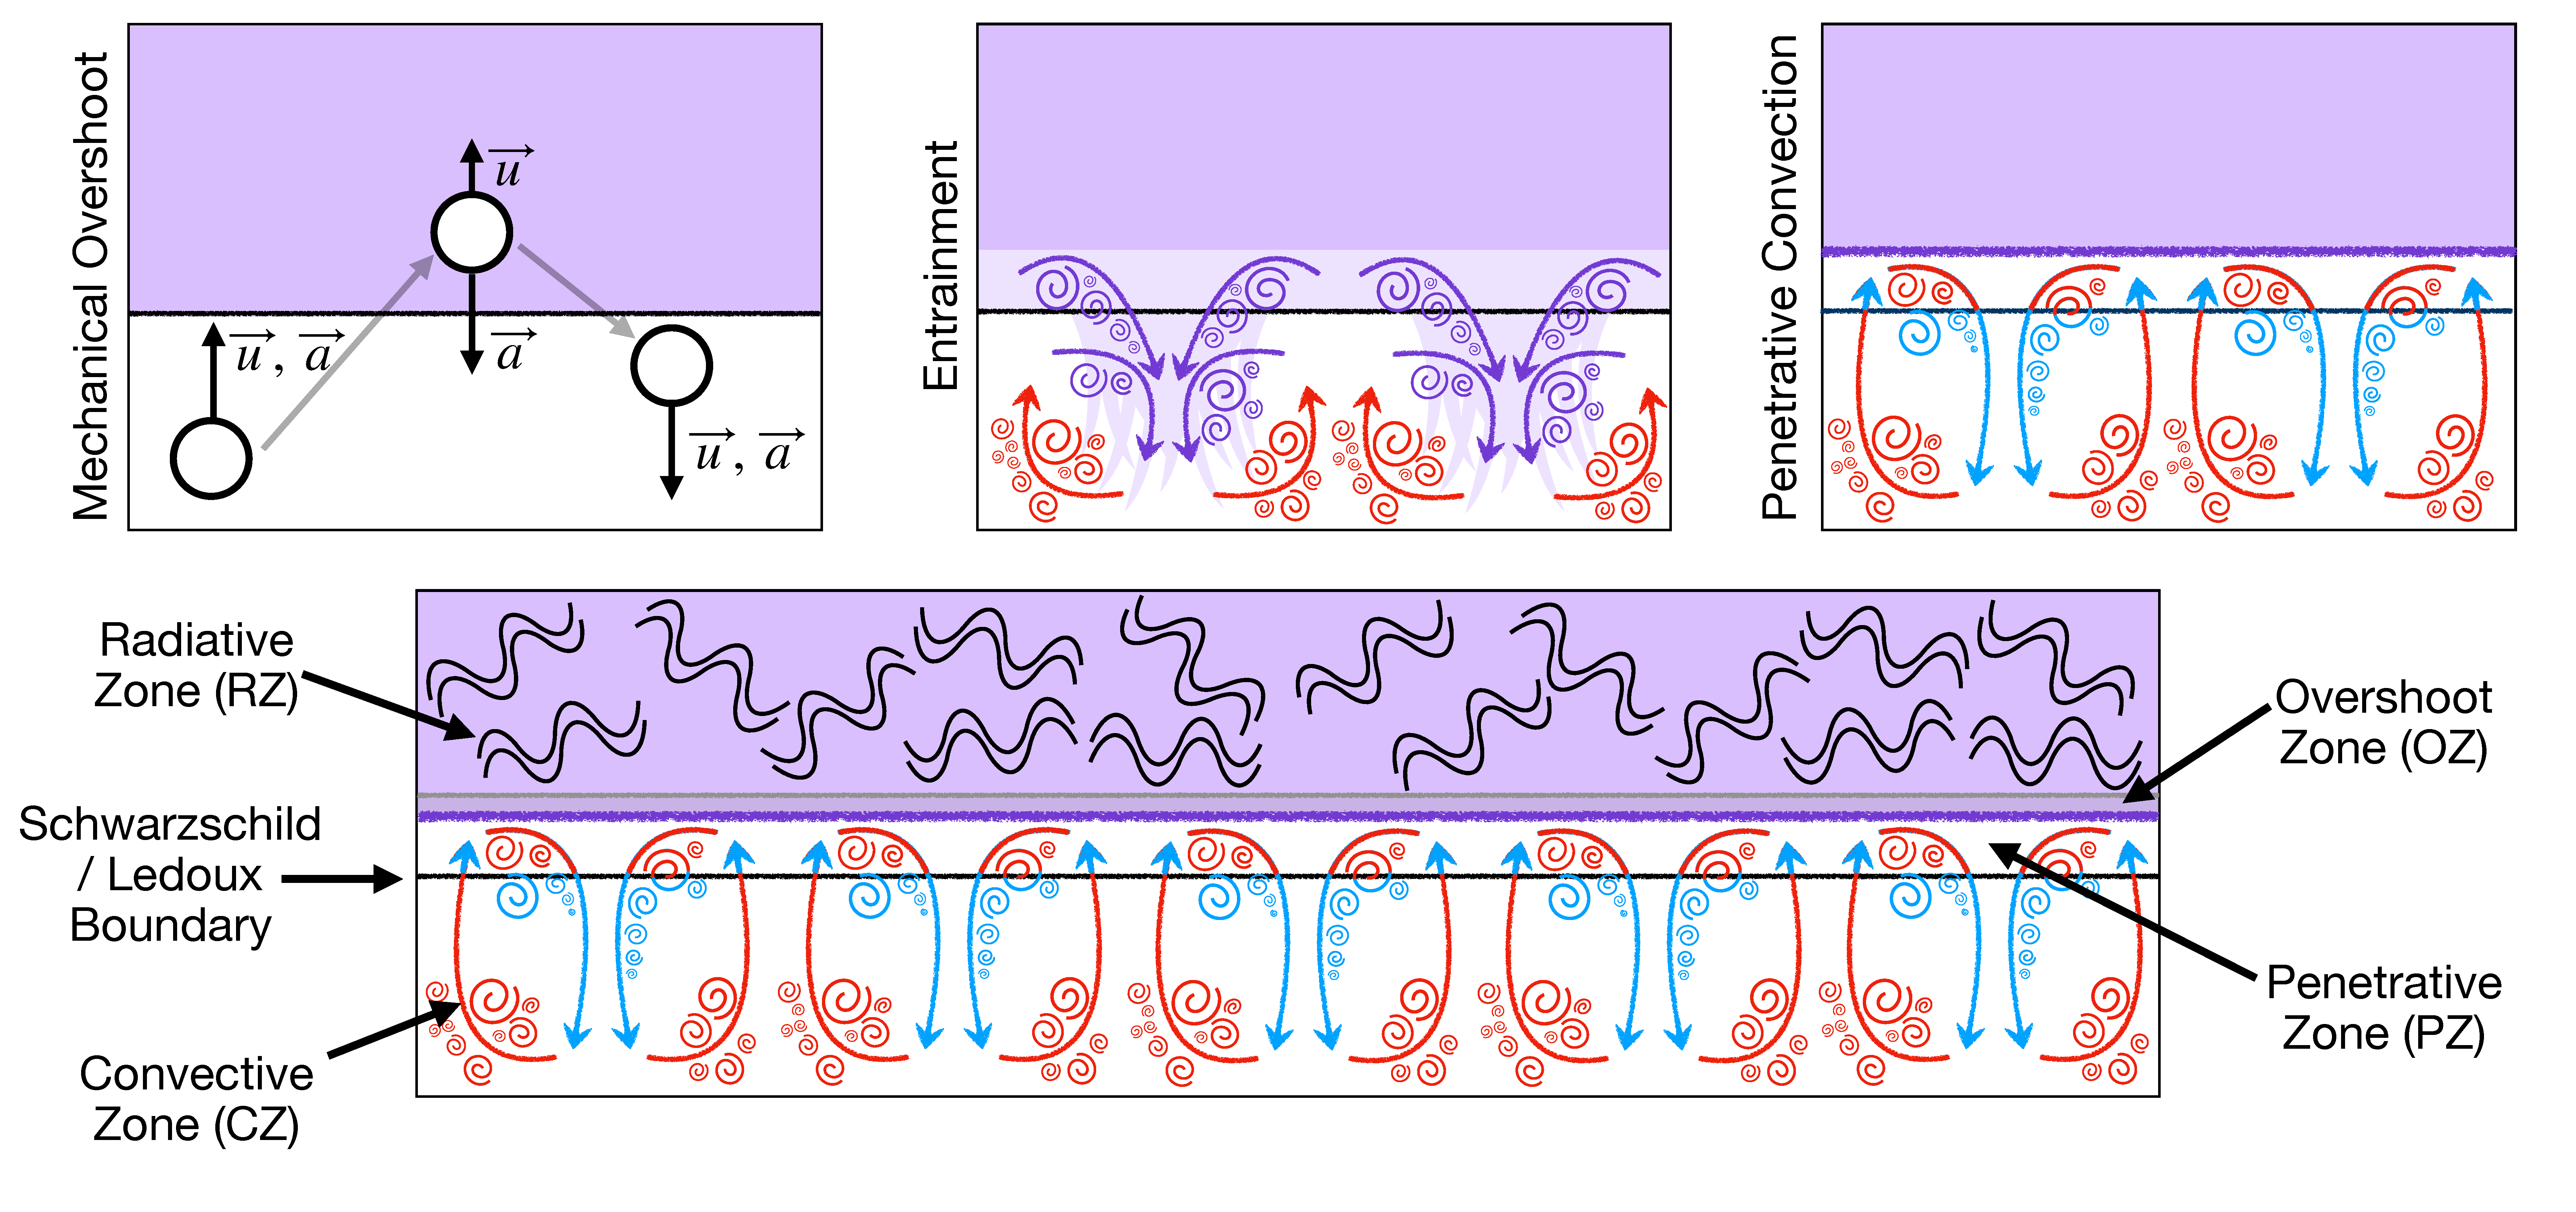
\includegraphics[width=\textwidth]{processes_and_structure_figure.pdf}
\caption{
    The three processes discussed in Sec.~\ref{sec:processes} are schematically demonstrated in the top row.
    White fluid has the properties of the well-mixed CZ, while purple fluid is the stable RZ.
    (Left) Convective overshoot occurs when a fluid parcel from the CZ crosses into the RZ; due to a strong positive entropy gradient in the RZ, the parcel is accelerated back into the CZ.
    (Middle) Motions generated by overshooting fluid parcels drag fluid from the RZ into the CZ in a process called entrainment.
    (Right) If a region of fluid beyond the convective boundary becomes well-mixed, it is a PZ; a divergence of the radiative flux acts as an internal cooling term, changing the buoyant signature of both upflows and downflows.
    In the bottom panel, we show the structure of a statistically-stationary convective boundary.
    The CZ sits below a well-mixed PZ.
    Above the PZ, the fluid is stable but there is a small OZ where convective overshoot occurs.
    Above this region is the stable RZ where there are internal gravity waves excited by the convection.
\label{fig:schema}
}
\end{figure*}





\subsection{Entrainment}
The process of entrainment is shown in the upper middle panel of Fig.~\ref{fig:schema}.
Return flows from overshooting convection carry fluid with the chemical and thermodynamic signature of the RZ.
This material then rapidly turbulently mixes in the convection zone.
As a result, convective motions which overshoot and entrain materials can gradually move convective boundaries.
Since entrainment is linked to convective overshooting, the overshoot distance $\Delta x$ directly relates to the \emph{rate} of entrainment; this statement can be inferred from entrainment rate laws \citep{meakin_arnett_2007} or interface flux arguments \citep{fuentes_cumming_2020}.

Entrainment has been modeled in 1D stellar evolution software instruments by \citet{staritsin_2013} and \citet{scott_etal_2021}, but their implementations differ from one another and entrainment is not standard in any instrument.


\subsection{Penetrative Convection}
The process of penetrative convection is shown in the upper right panel of Fig.~\ref{fig:schema}.
Through continual overshoot and entrainment, convection creates well-mixed regions beyond the convective boundary \citep{anders_etal_2021}.
These well-mixed extensions of the CZ are known as penetration zones (PZs).
Since PZs grow gradually over many dynamical times, they can extend beyond the overshoot distance $\Delta x$.

Penetrative convection most closely resembles ``step overshoot'' employed in 1D models, but penetrative convection mixes both entropy and composition.
